
\documentclass{article}

% -----------------------------
% Packages
% -----------------------------
\usepackage{fancyhdr}
\usepackage{extramarks}
\usepackage{amsmath}
\usepackage{amsthm}
\usepackage{amsfonts}
\usepackage{tikz}
\usepackage[plain]{algorithm}
\usepackage{algpseudocode}
\usepackage{amssymb}
\usepackage{graphicx}

\usetikzlibrary{automata,positioning}

% -----------------------------
% Basic Document Settings
% -----------------------------
\topmargin=-0.45in
\evensidemargin=0in
\oddsidemargin=0in
\textwidth=6.5in
\textheight=9.0in
\headsep=0.25in

\linespread{1.1}

\pagestyle{fancy}
\lhead{\hmwkAuthorName}
\chead{\hmwkClass: \hmwkTitle}
\rhead{}
\lfoot{\lastxmark}
\cfoot{\thepage}

\renewcommand\headrulewidth{0.4pt}
\renewcommand\footrulewidth{0.4pt}

\setlength\parindent{0pt}

% -----------------------------
% Problem Section Helpers
% -----------------------------
\newcommand{\enterProblemHeader}[1]{
  \nobreak\extramarks{}{Problem \arabic{#1} continued on next page\ldots}\nobreak{}
  \nobreak\extramarks{Problem \arabic{#1} (continued)}{Problem \arabic{#1} continued on next page\ldots}\nobreak{}
}

\newcommand{\exitProblemHeader}[1]{
  \nobreak\extramarks{Problem \arabic{#1} (continued)}{Problem \arabic{#1} continued on next page\ldots}\nobreak{}
  \stepcounter{#1}
  \nobreak\extramarks{Problem \arabic{#1}}{}\nobreak{}
}

\setcounter{secnumdepth}{0}
\newcounter{partCounter}
\newcounter{homeworkProblemCounter}
\setcounter{homeworkProblemCounter}{1}
\nobreak\extramarks{Problem \arabic{homeworkProblemCounter}}{}\nobreak{}

% -----------------------------
% Theorem env (optional)
% -----------------------------
\newtheorem*{theorem}{Theorem}

% -----------------------------
% Homework Problem Environment
%   Usage:
%   \begin{homeworkProblem}            % auto-number
%     % Your answer here
%   \end{homeworkProblem}
%
%   \begin{homeworkProblem}[7]         % set problem number to 7
%     % Your answer here
%   \end{homeworkProblem}
% -----------------------------
\newenvironment{homeworkProblem}[1][-1]{
  \ifnum#1>0
    \setcounter{homeworkProblemCounter}{#1}
  \fi
  \section{Problem \arabic{homeworkProblemCounter}}
  \setcounter{partCounter}{1}
  \enterProblemHeader{homeworkProblemCounter}
}{
  \exitProblemHeader{homeworkProblemCounter}
}

% -----------------------------
% Homework Details (EDIT THESE)
% -----------------------------
\newcommand{\hmwkTitle}{Homework \ 4}
\newcommand{\hmwkClass}{CS 4262}
\newcommand{\hmwkClassInstructor}{Prof. Dr. Thomas Beckers}
\newcommand{\hmwkAuthorName}{\textbf{Joseph Quinn}}

% -----------------------------
% Title
% -----------------------------
\title{
  \vspace{2in}
  \textmd{\textbf{\hmwkClass:\ \hmwkTitle}}\\
  \vspace{0.1in}\large{\textit{\hmwkClassInstructor\ }}
  \vspace{3in}
}
\author{\hmwkAuthorName}
\date{}

% -----------------------------
% Convenience Macros (optional)
% -----------------------------
\renewcommand{\part}[1]{\textbf{\large Part \Alph{partCounter}}\stepcounter{partCounter}\\}

% Algorithms
\newcommand{\alg}[1]{\textsc{\bfseries \footnotesize #1}}

% Calculus
\newcommand{\deriv}[1]{\frac{\mathrm{d}}{\mathrm{d}x} (#1)}
\newcommand{\pderiv}[2]{\frac{\partial}{\partial #1} (#2)}
\newcommand{\dx}{\mathrm{d}x}

% Statistics
\newcommand{\E}{\mathrm{E}}
\newcommand{\Var}{\mathrm{Var}}
\newcommand{\Cov}{\mathrm{Cov}}
\newcommand{\Bias}{\mathrm{Bias}}

% Proof step (for aligned derivations)
\newcommand{\step}[2]{& #1 & & \text{#2} \\}

% Solution header (optional)
\newcommand{\solution}{\textbf{\large Solution}}

% -----------------------------
% Document
% -----------------------------
\begin{document}

\maketitle
\pagebreak

\begin{homeworkProblem}

	\subsection*{1.1}

	This is an iterative algorithm for clustering
	\medskip

	Input: Data ${x^{(i)},\dots,x^{(N)} \in \mathbb{R}^d}$
	\medskip

	Output: Centroids ${u^{(i)},\dots,x^{(K)} \in \mathbb{R}^d}$
	\medskip

	Process:
	\begin{enumerate}
		\item Initilaize with K random centroids
		\item Repeat until convergence
		      \begin{itemize}
			      \item Assign a cluster to every sample $x^{(i)} \Rightarrow c^{(i)} = \arg\min_k dist(x^{(i)}, u^{(k)})$
			      \item Update centroids according to clusters: \[
				            \mu^{(k)} =
				            \frac{\displaystyle \sum_{i=1}^{N} \mathbf{1}_{c_i = k} \, x^{(i)}}
				            {\displaystyle \sum_{i=1}^{N} \mathbf{1}_{c_i = k}}
			            \]

		      \end{itemize}
	\end{enumerate}

	Now, the computational time complexity of this algorithm is made up of these parts:
	\begin{enumerate}
		\item Assign data points to closes centroid: $O(KN)$
		\item Change the cluster center to the average of its assigned points $O(N)$
	\end{enumerate}
	Lets say this loop occurs T times until convergence, then our final time complexity is $O(KNT)$
	\subsection*{1.2}

	\begin{figure}[h]
		\centering
		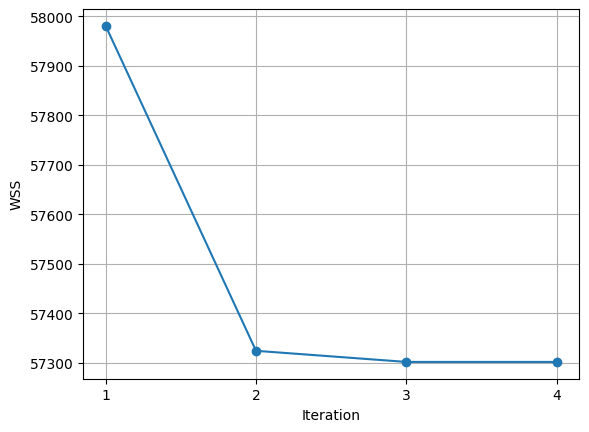
\includegraphics[width=0.5\textwidth]{../../imgs/hw4_1.2.png}
	\end{figure}
	\pagebreak

	\subsection*{1.3}

	\begin{figure}[ht]
		\centering
		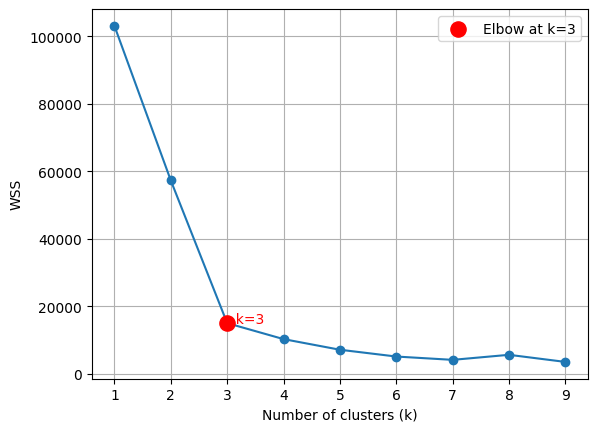
\includegraphics[width=0.5\textwidth]{../../imgs/hw4_1.3.png}
	\end{figure}

	Based on our results we see the optimal number of clusters based on the elbow method is 3, after which we get diminishing returns for each additional cluster.
	\subsection*{1.4}

	\begin{figure}[ht]
		\centering
		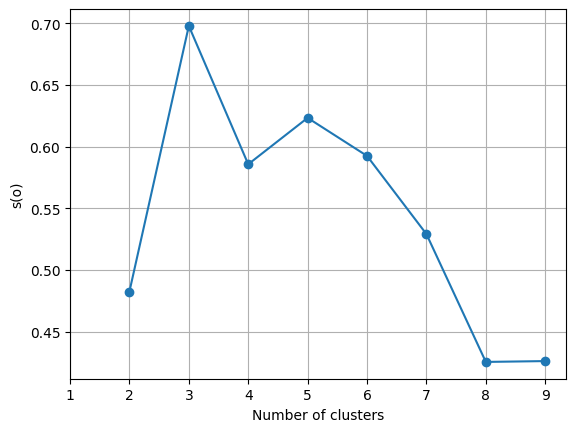
\includegraphics[width=0.5\textwidth]{../../imgs/hw4_1.4.png}
	\end{figure}

	Based on our results we can see that our optimal number of clusters based on the silhouette method is also 3 clusters as it has the highest silhouette coefficient.
\end{homeworkProblem}

\pagebreak

\begin{homeworkProblem}
	\subsection*{2.1}
	A Gaussian mixture model is a clustering algorithm that instead of clustering by geometric distances, clusters with a mixture of gaussian distributions.
	Also, unlike K-Means (which assigns points to a single cluster), GMM gives soft assignments using probabilities.

	\medskip

	A Gaussian Mixture Model assumes that the data is generated by a mixture (i.e., combination) of $K$ Gaussian distributions:

	\[
		p(x;\{(\alpha_k,\mu_k,\sigma_k)\}_{k=1}^{K})
		= \sum_{k=1}^{K} \alpha_k \, \mathcal{N}(x;\mu_k,\sigma_k)
		= \sum_{k=1}^{K} \frac{\alpha_k}{\sqrt{2\pi\sigma_k^2}}
		\exp\left( -\frac{(x - \mu_k)^2}{2\sigma_k^2} \right)
	\]

	where
	\[
		\alpha_k \ge 0, \quad \sum_{k=1}^{K} \alpha_k = 1
	\]
	are the mixing coefficients, and $\mu_k, \sigma_k$ are the mean and standard deviation of each Gaussian component.

	\medskip

	Our optimization problem is that given the data $\{x^{(1)}, x^{(2)}, \dots, x^{(N)}\}$, we want to estimate the parameters
	\[
		\Theta = \{(\alpha_k,\mu_k,\sigma_k)\}_{k=1}^{K}
	\]
	by maximizing the log-likelihood:

	\[
		\mathcal{L}(\Theta)
		= \sum_{i=1}^{N} \log \left(
		\sum_{k=1}^{K} \alpha_k \, \mathcal{N}(x^{(i)};\mu_k,\sigma_k)
		\right)
	\]

	Since this objective has no closed-form solution, it is optimized using the Expectation-Maximization (EM) algorithm.

	\subsection*{2.2}
	The EM algorithm consists of 2 steps:

	\begin{itemize}
		\item \textbf{E-Step (Expectation):} Compute the probability that each data point belongs to each component (soft assignments).
		\item \textbf{M-Step (Maximization):} Update the parameters to maximize the expected log-likelihood based on the soft assignments.
	\end{itemize}

	\paragraph*{E-Step: Compute Responsibilities}

	For fixed parameters $\{(\alpha_k, \mu_k, \sigma_k)\}_{k=1}^{K}$, compute the \textbf{responsibility} $r_n^k$ for each data point $x_n$ and each component $k$:

	\[
		r_n^k = p(z_k = 1 \mid x_n)
		= \frac{ \alpha_k \, \mathcal{N}(x_n; \mu_k, \sigma_k^2) }
		{ \sum\limits_{i=1}^{K} \alpha_i \, \mathcal{N}(x_n; \mu_i, \sigma_i^2) }
	\]

	This is the probability that data point $x_n$ was generated by component $k$.

	\paragraph*{M-Step: Update Parameters}

	For fixed responsibilities $r_n^k$, update the parameters as follows:

	\medskip

	\textbf{1. Update Mixture Coefficients}

	\[
		\alpha_k = \frac{N_k}{N}
		\; \; \text{for} \; \;
		N_k = \sum_{n=1}^{N} r_n^k
	\]

	\textbf{2. Update Means}

	\[
		\mu_k = \frac{1}{N_k} \sum_{n=1}^{N} r_n^k x_n
	\]

	\textbf{3. Update Covariances}

	\[
		\Sigma_k = \frac{1}{N_k} \sum_{n=1}^{N} r_n^k (x_n - \mu_k)(x_n - \mu_k)^T
	\]

	Repeat the E-step and M-step until the log-likelihood converges (or changes very little), or until a maximum number of iterations is reached.

\end{homeworkProblem}

\subsection*{2.3}


\begin{figure}[!ht]
	\centering
	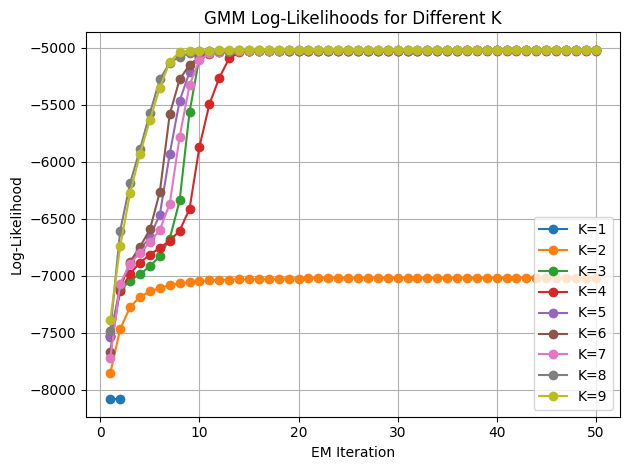
\includegraphics[width=0.48\textwidth]{../../imgs/hw4_2.31.png}
	\qquad
	\begin{tabular}[b]{cc}
		\hline
		\textbf{K} & \textbf{Final Log-Likelihood} \\
		\hline
		1          & -8083.98                      \\
		2          & -7020.47                      \\
		3          & \textbf{-5029.02}             \\
		4          & -5025.82                      \\
		5          & -5024.24                      \\
		6          & -5023.32                      \\
		7          & -5020.56                      \\
		8          & -5018.60                      \\
		9          & -5021.33                      \\
		\hline
	\end{tabular}
\end{figure}
I would say 3 clusters would be the best candidate as we do not see a noticeable increase in performance when increasing cluster count further.

\end{document}
